\documentclass[a4paper]{paper}

\usepackage[catalan]{babel}
\usepackage{fontspec}
\usepackage[margin=2cm]{geometry}

\usepackage{graphicx}
\usepackage{float}

\usepackage{listings}

\usepackage[colorlinks=true, allcolors=blue, linkcolor=black]{hyperref}

\usepackage{xcolor}
\usepackage{tikz}

\usepackage[
backend=biber,
citestyle=numeric  
]{biblatex}

\newcommand*{\framemargin}{3ex}
\newcommand*{\literatecolour}{\textcolor{literatecolour}}
\newcommand*{\pythonprompt}{\textcolor{promptcolour}{{>}{>}{>}}}

\definecolor{gray}{gray}{0.5}
\colorlet{commentcolour}{green!50!black}
\colorlet{stringcolour}{red!60!black}
\colorlet{keywordcolour}{magenta!90!black}
\colorlet{exceptioncolour}{yellow!50!red}
\colorlet{commandcolour}{blue!60!black}
\colorlet{numpycolour}{blue!60!green}
\colorlet{literatecolour}{magenta!90!black}
\colorlet{promptcolour}{green!50!black}
\colorlet{specmethodcolour}{violet}

\lstdefinestyle{mypython}{
	numbers=left,
	language=python,
	showtabs=true,
	tab=,
	tabsize=2,
	basicstyle=\ttfamily\footnotesize,%\setstretch{.5},
	stringstyle=\color{stringcolour},
	showstringspaces=false,
	alsoletter={1234567890},
	otherkeywords={\%, \}, \{, \&, \|},
	keywordstyle=\color{keywordcolour}\bfseries,
	emph={and,break,class,continue,def,yield,del,elif ,else,%
		except,exec,finally,for,from,global,if,import,in,%
		lambda,not,or,pass,print,raise,return,try,while,assert,with},
	emphstyle=\color{blue}\bfseries,
	emph={[2]True, False, None},
	emphstyle=[2]\color{keywordcolour},
	emph={[3]object,type,isinstance,copy,deepcopy,zip,enumerate,reversed,list,set,len,dict,tuple,xrange,append,execfile,real,imag,reduce,str,repr},
	emphstyle=[3]\color{commandcolour},
	emph={Exception,NameError,IndexError,SyntaxError,TypeError,ValueError,OverflowError,ZeroDivisionError},
	emphstyle=\color{exceptioncolour}\bfseries,
	morecomment=[s]{"""}{"""},
	commentstyle=\color{commentcolour}\slshape,
	emph={[4]ode, fsolve, sqrt, exp, sin, cos,arctan, arctan2, arccos, pi,  array, norm, solve, dot, arange, isscalar, max, sum, flatten, shape, reshape, find, any, all, abs, plot, linspace, legend, quad, polyval,polyfit, hstack, concatenate,vstack,column_stack,empty,zeros,ones,rand,vander,grid,pcolor,eig,eigs,eigvals,svd,qr,tan,det,logspace,roll,min,mean,cumsum,cumprod,diff,vectorize,lstsq,cla,eye,xlabel,ylabel,squeeze},
	emphstyle=[4]\color{numpycolour},
	emph={[5]__init__,__add__,__mul__,__div__,__sub__,__call__,__getitem__,__setitem__,__eq__,__ne__,__nonzero__,__rmul__,__radd__,__repr__,__str__,__get__,__truediv__,__pow__,__name__,__future__,__all__},
	emphstyle=[5]\color{specmethodcolour},
	emph={[6]assert,yield},
	emphstyle=[6]\color{keywordcolour}\bfseries,
	emph={[7]range},
	emphstyle={[7]\color{keywordcolour}\bfseries},
	literate=*%
	{:}{{\literatecolour:}}{1}%
	{=}{{\literatecolour=}}{1}%
	{-}{{\literatecolour-}}{1}%
	{+}{{\literatecolour+}}{1}%
	{*}{{\literatecolour*}}{1}%
	{**}{{\literatecolour{**}}}2%
	{/}{{\literatecolour/}}{1}%
	{//}{{\literatecolour{//}}}2%
	{!}{{\literatecolour!}}{1}%
	%{(}{{\literatecolour(}}{1}%
	%{)}{{\literatecolour)}}{1}%
	{[}{{\literatecolour[}}{1}%
	{]}{{\literatecolour]}}{1}%
	{<}{{\literatecolour<}}{1}%
	{>}{{\literatecolour>}}{1}%
	{>>>}{\pythonprompt}{3}%
	,
	rulecolor=\color{black!40},
	backgroundcolor=\color{white},
	breakindent=.5\textwidth,frame=single,breaklines=true,
}



\setlength{\parindent}{0pt}
\setlength{\parskip}{0.5em}
\def\arraystretch{1.5}

\nocite{*}
\bibliography{bibliografia.bib}

\let\oldsection\section
\renewcommand\section{\clearpage\oldsection}
\renewcommand{\lstlistingname}{Codi}

\begin{document}

\begin{titlepage}
	\centering
	\vspace{1cm}
	
\includegraphics[width=0.25\textwidth]{images/etseib}
	\par\vspace{1cm}
	\textsc{ \LARGE Escola Tècnica Superior d'Enginyeria \\[1em] 
		Industrial de Barcelona}
	\par\vspace{2cm}
	\textbf{\LARGE Projecte II}
	\par\vspace{2cm}
	{\Huge Construcció d'una orquestra amb Raspberry Pi}
	\vfill
	\begin{flushright}
		\large
		Arnau Canyadell i Miquel \par
		Joan Marcè i Igual \par
	\end{flushright}
\end{titlepage}

\tableofcontents

\newpage

\section{Introducció}

\subsection{Motivacions}

Els dos creadors d'aquest projecte hem realitzat diversos estudis de música i, a més a més, hem participat algun cop en una orquestra. També, com a estudiants d'enginyeria industrial i informàtica que som, ens apassiona la tecnologia.

Així doncs, s'ha decidit intentar combinar aquestes dues motivacions i crear una orquestra que sigui interpretada i dirigida mitjançant tecnologia completament. S'usen Raspberry Pis ja que són dispositius molt versàtils i perfectament aptes per aquesta tasca. Aquests estan connectats entre ells mitjançant \emph{multicast} de manera que n'hi ha un que fa el rol de director i els altres el d'intèrpret.

\subsection{Projectes similars}

Buscant si hi ha altres projectes semblants al que es vol realitzar s'ha trobat que Google l'any 2011 va crear el projecte \emph{YouTube Symphony Orchestra 2011}\cite{YoutubeSymphoni} que tenia com a objectiu poder fer una orquestra a nivell mundial. Per fer-ho tots els músics es connectaven a internet i després tocaven tots junts i tot seguit totes les pistes d'àudio que aquests generaven s'ajuntaven formant una orquestra.

A part també hi ha un projecte anomenat \emph{Orchestra! a Distributed Platform for Virtual Musical Groups and Music Distance Learning over the Internet in Java \texttrademark Technology} \cite{Orchestra}. Que permet a diversos grups de música assajar o aprendre conjuntament a través d'internet tot i que no es trobin junts físicament.

\section{Objectius}
A l'inici del projecte es van establir uns objectius a complir en el projecte. Aquests es van dividir en dos grups. D'una banda, els objectius a curt termini, objectius que estaven ben definits i s'havien de fer sí o sí abans que s'acabés el projecte; i d'altra banda hi havia els objectius o idees a llarg termini, que no estaven tan ben definits i que s'intentarien completar si hi havia temps.

\subsection{Objectius a curt termini}
\begin{itemize}
	\item Aconseguir rebre la música d'un ordinador
	\item Enviar la música a una Raspberry Pi
	\item Reproduir la música en una Raspberry Pi
\end{itemize}

\subsection{Objectius a llarg termini}
\begin{itemize}
	\item Programar un bot per a l'aplicació de missatgeria Te\textit{}legram que reprodueixi amb l'orquestra de Raspberry Pis la música que se li enviï.
	\item Enviar música del mòbil a l'ordinador.
\end{itemize}

\section{Desenvolupament del treball}
El treball s'ha dut a terme durant un el quadrimestre de primavera, des de mitjans de febrer fins a finals de maig. S'ha estructurat la feina en 14 sessions, fent defenses parcials del projecte a les sessions 5 i 9, i una defensa final en l'última.

\subsection{Eines de treball}
Degut a ala naturalesa de desenvolupament de programari informàtic del projecte i de la necessitat de mantenir un historial de versions i un ordre del codi, s'ha treballat amb un \textbf{repositori públic de GitHub} (\url{https://github.com/jmigual/projecte2/}).

Per a l'assignació de tasques dintre del grup s'ha utilitzat l'eina Trello\cite{trello}, que permet crear tasques amb data límit, assignar-les a una persona i marcar tasques com a realitzades o endarrerides, entre altres coses.

Per al desenvolupament del programari s'ha utilitzat majoritàriament el llenguatge Python\cite{python}, amb el qual està fet tot el codi de l'orquestra, inclosos director, músics i bot. S'ha utilitzat l'entorn de Pycharm\cite{pycharm} per a escriure codi, executar-lo i depurar-lo en aquest llenguatge. Per a la configuració de les Raspberry Pis s'ha utilitzat shell script, i també s'ha treballat molt amb comandes de git.

Finalment, totes les presentacions del projecte i la memòria s'han fet amb \LaTeX.

\subsection{Evolució del projecte}
En el repositori hi ha el document \texttt{Documentacio.md} on es detalla l'historial de feina feta en cada sessió (començant en la sessió 3).

\subsubsection{Inici (sessions 1 a 3)}
En les primeres sessions es va decidir el tema i es van establir els objectius del projecte. També es van definir les eines de treball que s'utilitzarien durant el projecte: es va crear el repositori a GitHub i es va crear el Trello. D'altra banda, es va buscar documentació sobre el FluidSynth i el Polyphone i es va analitzar el codi del director que ja estava implementat. Finalment, es va aprendre a configurar la Raspberry Pi i es va configurar la raspberry que s'ha utilitzat per fer les proves al llarg de tot el desenvolupament.

\subsubsection{Programació del director i els músics (sessions 4 a 9)}
Un cop endinsats en el projecte, es va començar a desenvolupar el programari. Es va programar, primer de tot, una versió del músic, que rebia la música del director i la reproduïa. En aquest punt es va trobar un problema amb la configuració de la sortida d'àudio de la Raspberry Pi: la sortida per defecte és el minijack, i no se sabia com canviar-la a la targeta USB. Per tal de solucionar-ho es va provar de canviar diverses configuracions, i finalment es va optar per instal·lar pixel a l'ordinador monoplaca i canviar la configuració manualment des de l'entorn gràfic. Així es va aconseguir solucionar el problema però el canvi implicava connectar-se manualment a l'entorn gràfic cada cop que s'iniciava la Raspberry Pi.

Un cop tot funcionava es modificar el director. Es van crear les classes Director i Nota per separar, ordenar i simplificar el codi. En la segona defensa del projecte, a la sessió 9, es va poder dur a terme la primera prova de l'orquestra amb diversos músics. Al final d'aquesta fase del treball ja s'havien complert els objectius a curt termini.

\subsubsection{Implementació del bot de Telegram i reproducció d'arxius MIDI (sessions 10 a 14)}
Finalment es va trobar una manera de canviar la sortida d'àudio de les Raspberry Pis i es va crear un script per canviar-lo de forma simplificada. Després d'això es va treballar en l'objectiu de crear un bot de Telegram que reproduís la música que se li envia, i així complir els dos objectius a llarg termini. Per a dur a terme aquest objectius es va para\l.lelitzar la feina en la creació del bot i en la reproducció d'arxius MIDI.

\section{Funcionament de l'orquestra}

\subsection{Comunicació entre director i intèrprets}
Per al funcionament de la orquestra hi ha un dispositiu que fa de director i la resta de dispositius fan d'intèrprets, tots ells són Raspberry Pis.

Per al funcionament de la comunicació s'ha usat multicast. El funcionament és el següent: els clients es subscriuen a una IP en concret i quan algú envia dades a aquesta IP llavors el router reenvia aquestes dades a tots els dispositius que s'han subscrit.

\begin{figure}[H]
	\centering
	\def\width{.1\textwidth}
	\begin{tikzpicture}
		\node[
			label = left:{Router}]
			(router){
\includegraphics[width=\width]{images/cisco/router}};
		\node[
			below = of router, 
			label = left:{Switch}] 
			(switch){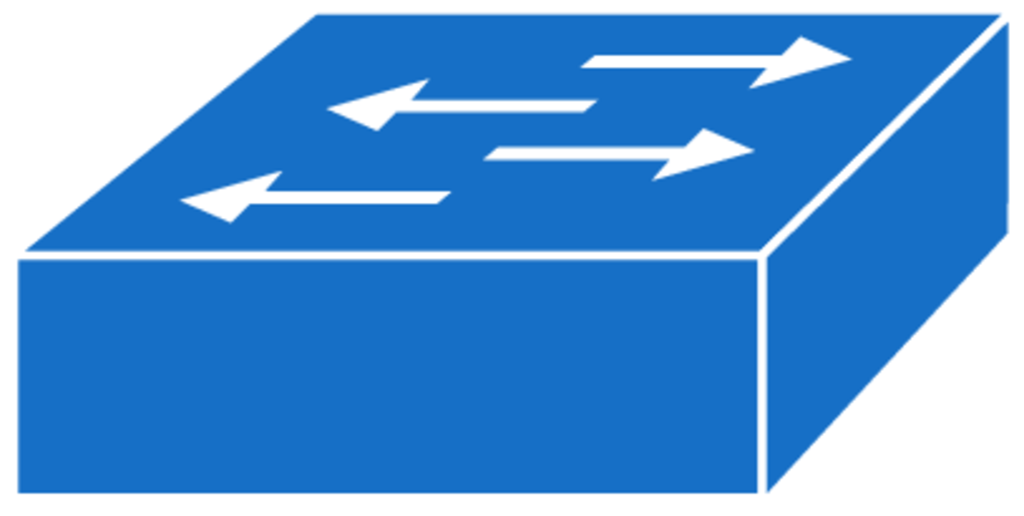
\includegraphics[width=\width]{images/cisco/workgroup_switch} };
		\node[
			below left = of switch,
			label = below:{Director}]
			(director){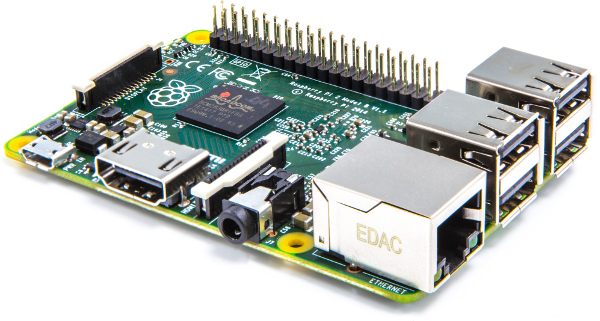
\includegraphics[width=\width]{images/raspberry}};
		\node[
			below right = of switch,
			label = below:{Músic 1}]
			(m1){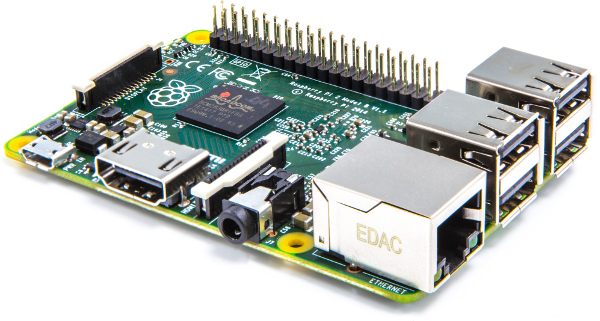
\includegraphics[width=\width]{images/raspberry}};
		\node[
			right = of m1,
			label = below:{Músic 2}]
			(m2){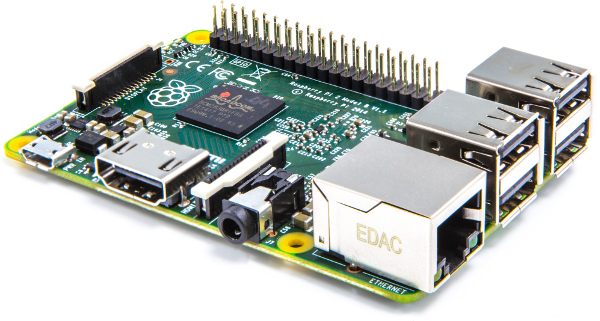
\includegraphics[width=\width]{images/raspberry}};
		\node[
			right = of m2,
			label = below:{Músic 3}]
			(m3){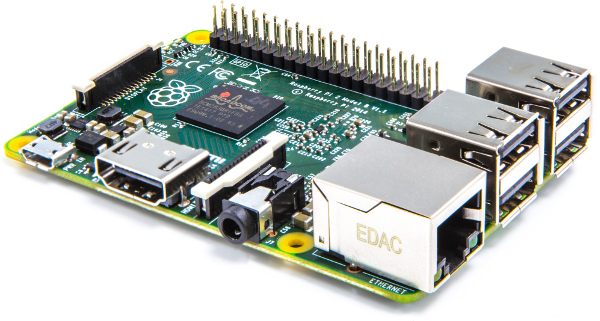
\includegraphics[width=\width]{images/raspberry}};	
		
		\draw[latex-latex] (router) -- (switch);
		\draw[-latex] (director) -- (switch);
		\draw[-latex] (switch) -- (m1);
		\draw[-latex] (switch) -- (m2);
		\draw[-latex] (switch) -- (m3);
	\end{tikzpicture}
	\caption{Esquema de funcionament de la xarxa}
\end{figure}

\subsection{Bot de Telegram}
Telegram\cite{telegram} és una aplicació de missatgeria per a mòbils de diversos sistemes operatius i amb versions també per a ordinadors que admet un tipus concret d'usuaris que són bots. Aquests bots utilitzen una API proveïda per Telegram que els permet rebre i enviar missatges i contingut multimèdia amb els usuaris de l'aplicació.

El bot s'anomena \emph{Raspberry Pi Orchestra} i té l'identificador \texttt{@RPOrchestraBot}. El seu codi per a funcionar es troba al repositori del treball a la carpeta \texttt{Code} (\texttt{bot.py}) i es pot executar en qualsevol ordinador que tingui intèrpret de Python3 i connexió a Internet.

Cada vegada que un usuari envia un arxiu al bot, aquest comprova que sigui un arxiu de format MIDI. Si ho és, l'envia al director perquè el toqui amb l'orquestra de Raspberry Pis. Actualment la funció que executa aquest codi és síncrona i no acaba fins que l'orquestra de tocar. Això significa que el bot no reacciona a cap missatge que li sigui enviat mentre l'orquestra està tocant, i per tant si un usuari envia un nou arxiu MIDI aquest no serà reproduït fins que la peça acabi. A la \autoref{fig:screenshot_bot} es pot veure un exemple de com funciona.

\begin{figure}
	\centering
	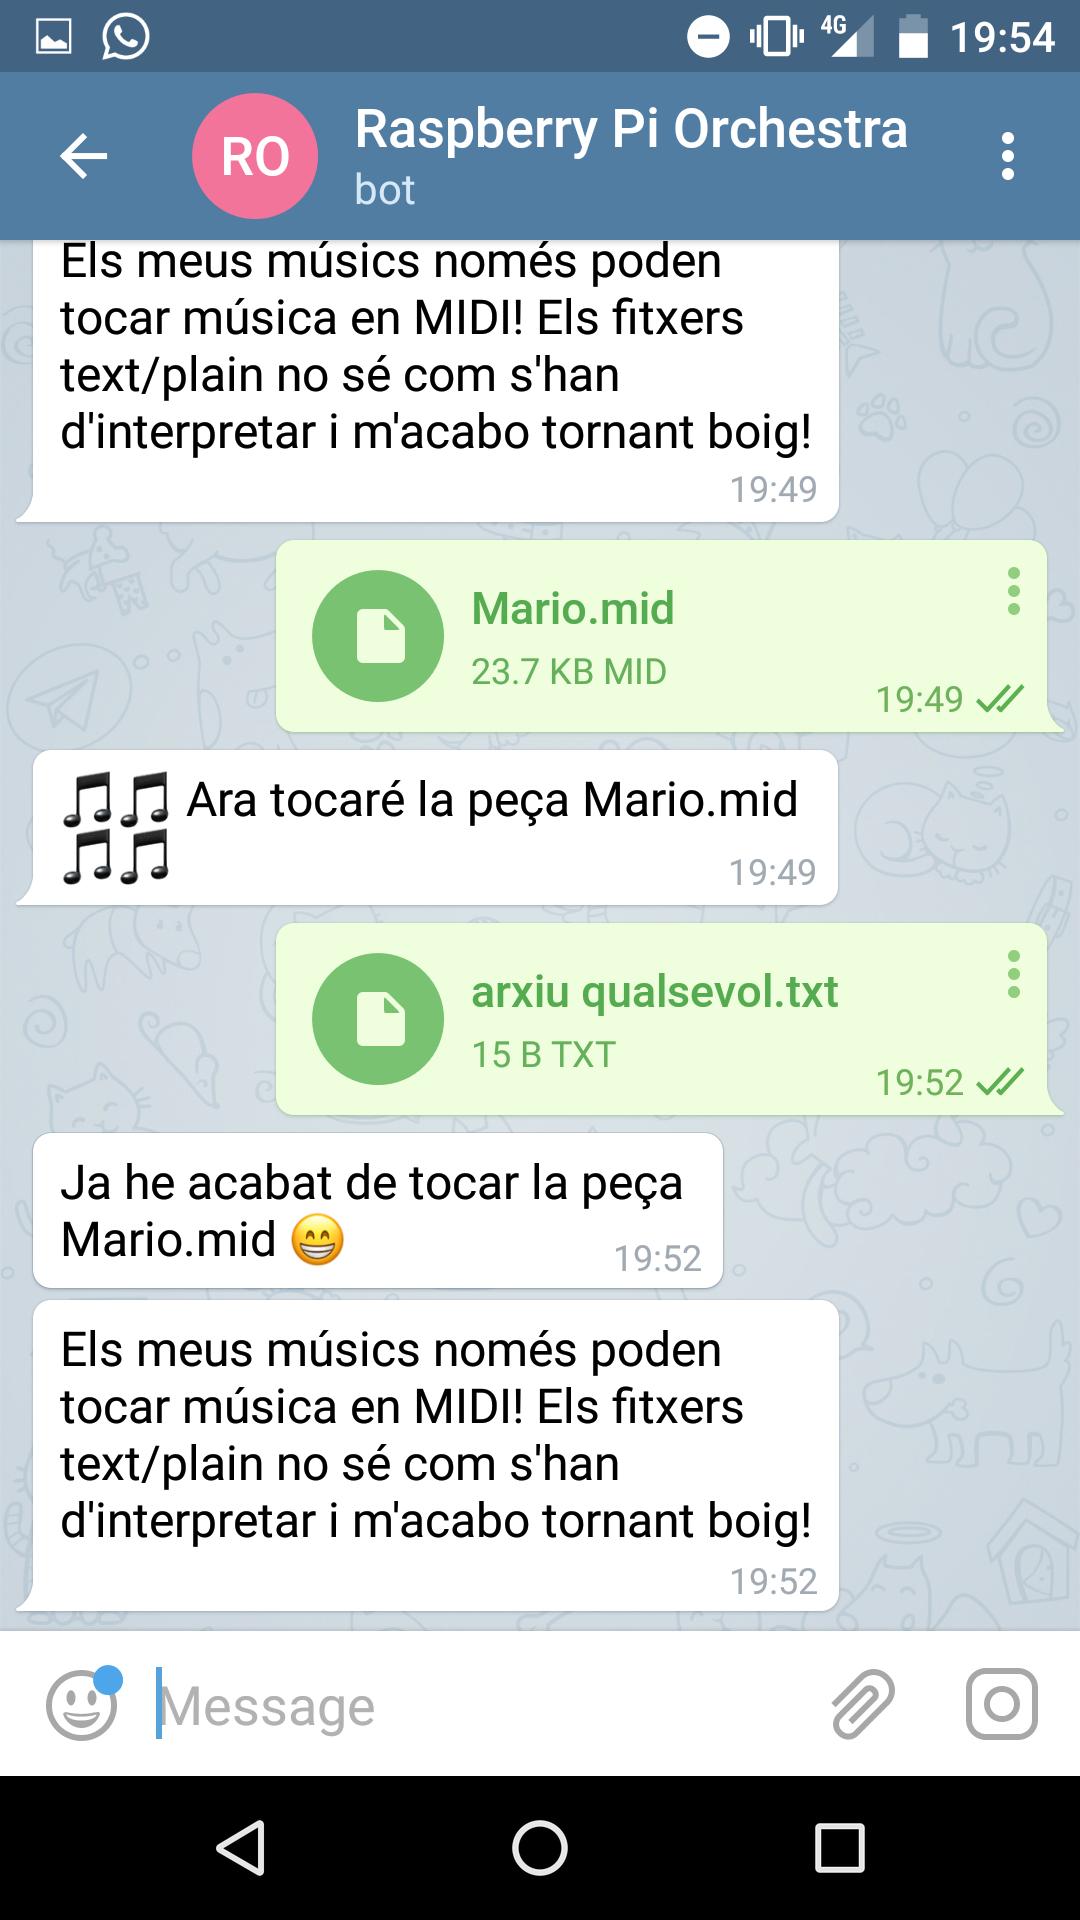
\includegraphics[width=0.3\textwidth]{images/screenshot_bot.png}
	\caption{Exemple d'interacció amb el \emph{Raspberry Pi Orchestra}. El bot no respon fins que l'orquestra no acaba de tocar la peça. Tambés es pot observar que no accepta l'arxiu que no és del tipus adequat.}
	\label{fig:screenshot_bot}
\end{figure}

El bot s'ha creat a partir d'una plantilla pública de codi lliure anomenada Python Telegram Bot\cite{python-telegram-bot}. Aquesta plantilla ofereix moltes classes per a realitzar les operacions de connexió amb els servidors de Telegram.

\subsection{Reproducció d'arxius MIDI}
Per a la reproducció dels arxius MIDI s'ha usat la llibreria Mido\cite{mido}. Que permet la reproducció en temps real d'aquest tipus d'arxius. Aquesta llibreria s'ha modificat lleugerament per poder obtenir tots els canals del MIDI mentre es reprodueix de manera que pot ser configurat amb el sistema de múltiples Raspberry Pi per reproduir que s'usa en aquest projecte.

Així doncs, un cop la connexió amb el bot de Telegram està finalitzada és tant senzill com passar el camí fins a l'arxiu que es vulgui reproduir i el nou director s'encarrega de demanar-li a la llibreria la informació necessària.

Una versió simplificada del codi és la que es pot veure al \autoref{lst:code}.
\begin{lstlisting}[
		float,
		label={lst:code},
		style=mypython, 
		xleftmargin=.1\textwidth, 
		xrightmargin=.1\textwidth,
		captionpos=b,
		caption={Bucle bàsic per enviar les dades de notes}
		]
	# file_path: conté el camí fins a l'arxiu
	# multicast_group: conté la ip al grup de multicast
	# La funció play_tracks() ja fa les pauses que s'hagin de fer perquè
	# les notes sonin quan toca
	mid = DirectorMidiFile(file_path)
	for missatge, track in mid.play_tracks():
		msg_in, msg_out = descodifica(missatge)
		# Genera string a enviar
		json_string = json.dumps({
		"in": msg_in,
		"out": msg_out
		})
	
		# Enviar dades al multicast
		socket.sendto(json_string.encode(), multicast_group)
\end{lstlisting}	

\section{Conclusions}
Pel que fa al treball, podem dir que hem assolit les metes que ens havíem proposat. Els dos objectius a llarg plaç s'han acabat podent implementar dins del termini i el resultat ha estat una aplicació que funciona sense problemes greus. A més, el projecte inclou el codi per configurar l'orquestra en altres noves Raspberry Pis, la qual cosa farà que el treball no mori quan s'hagi de retornar el material a final de curs, sinó que es pot tornar a muntar en un altre lloc. A més a més, tot el procés està detalladament documentat perquè qui ho vulgui pugui fer-ne ús.

D'altra banda, personalment els autors estem satisfets amb aquest treball perquè ens ha permès aprofundir en temes de programació molt diversos i enfrontar-nos a diversos reptes. Hem après en moltes àrees diverses de la informàtica:

\begin{itemize}
	\item Configuració de Raspberry Pis
	\item Python amb classes
	\item Creació de bots per a Telegram
	\item Conversió d'arxius a MIDI
	\item Comunicació en xarxa utilitzant Python
	\item Fer presentacions i redactar memòries utilitzant \LaTeX
	\item Ús d'una eina de control de versions
\end{itemize}

A part d'això, també hem pogut desenvolupar les "soft skills" de treball en grup i parlar en públic.


\printbibliography

\end{document}